\documentclass[
  utf8,%     More capable input encoding than latin-1.
  % parskip,%  For vertical whitespace between paragraphs.  This comes down to more than just using parskip.sty, so it's better to use this class option.
  % S5MP % If you intend to really use margin paragraphs (not recommended!).
%  crop,%     Produce output with crop marks and paper size A4.  Liu-Tryck should like this.  Automatically adds information, including the physical page number, at the top of each page.
       %     Add option 'noInfo' to suppress the info at the top of each page when using option 'crop'.
  % Font options: 'kp' (default), 'times', 'lm'.  The KpFonts (loaded using 'kp'), is the most complete font among the provided options.  Among other, it supports slanted small caps.  See rtthesis.cls for more details regarding the font options.
  largesmallcaps,intlimits,widermath,% Good options to KpFonts.
  sharecounter,nobreak,definition=marks,%  See comments in the results chapter of this document for more information on these options!
  numbers, % If you want to cite references by numbers, use this option.
  noparts, % Use option 'noparts' if you do not make use of part divisions.
]{rtthesis}

\usepackage{epstopdf}
\epstopdfsetup{update} % only regenerate pdf files when eps file is newer
\usepackage{mythesis}

% !TEX program = pdflatex
% !TEX root = main.tex

\begin{document}
\selectlanguage{english}

\frontmatter
\maketitle

%\begin{abstract}[swedish]
%  \input{svensk-sammanfattning}
%\end{abstract}

\begin{abstract}[english]
  The Equipment Controls and Electronics section at \abbrCERN is developing a high precision piezo-actuated rotational stage for the UA9 crystal collimation project. Several control-related issues arising from the complexity and operational environment of the system make it difficult to design a controller that achieves the desired performance. This thesis has investigating in different control approaches aiming to improve the tracking capability of the rotational stage. This thesis has shown that an \abbrIRC method can be used efficiently to attenuate the first resonance mode and to increase the closed loop bandwidth. It also showed that harmonic cancellation can be used to efficiently damp out known harmonic disturbances. Finally a feedforward harmonic cancellation method (\abbrRFDC) was implemented and proposed as an add-on to the present control algorithm.

%If your thesis is written in English, the primary abstract would go here while the Swedish abstract would be optional.

\end{abstract}

%\begin{acknowledgments}
  First of all, I would like to thank \abbrCERN and the \abbrENSTIECE section for giving me this opportunity. 

  \addvspace{1em}
  \begin{flushright}
    \textit{%
      Linköping, Augusti 2016\\
      Niklas Ericson%
    }
  \end{flushright}
\end{acknowledgments}


\tableofcontents
\begin{notation}% Passing the option "old" to the notation environment will redefine the notationtabular environment so that it produces an old style LaTeX tabular instead of a ctable.sty style tabular.
  \centering
  \begin{notationtabular}{Abbreviations}{Abbreviation}{Meaning}
    \abbrCERN\index{CERN@\abbrCERN!abbreviation} & European Organization for Nuclear Research \\
    \abbrENSTIECE\index{ENSTIECE@\abbrENSTIECE!abbreviation} & Equipment and Constrol Section - Source, Target and Interaction group - Engineering Department \\
    \abbrSTM\index{STM@\abbrSTM!abbreviation} & Scanning Tunneling Microscope \\
    \abbrAFM\index{AFM@\abbrAFM!abbreviation} & Atomic Force Microscope \\
    \abbrLHC\index{LHC@\abbrLHC!abbreviation} & Large Hadron Collider \\
    \abbrPEA\index{PEA@\abbrPEA!abbreviation} & Piezoelectric Actuator \\
    \abbrPID\index{PID@\abbrPID!abbreviation} & Proportional, Integral, Derivative (controller) \\
    \abbrDOF\index{DOF@\abbrDOF!abbreviation} & Degrees of Freedom \\
    \abbrPRBS\index{PRBS@\abbrPRBS!abbreviation} & Pseudo Random Binary Sequence \\
    \abbrTF\index{TF@\abbrTF!abbreviation} & Transfer Function \\
    \abbrQFT\index{QFT@\abbrQFT!abbreviation} & Quantitative Feedback Theorem \\
    \abbrFFT\index{FFT@\abbrFFT!abbreviation} & Fast Fourier Transform \\
    \abbrIRC\index{IRC@\abbrIRC!abbreviation} & Integral Resonance Control \\
    \abbrIMP\index{IMP@\abbrIMP!abbreviation} & Internal Model Principle \\
    \abbrRFDC\index{RFDC@\abbrRFDC!abbreviation} & Repetitive Feedforward Disturbance Cancellation \\
    \abbrMRAC\index{MRAC@\abbrMRAC!abbreviation} & Model Reference Adaptive Controller \\
    \abbrMRACPE\index{MRACPE@\abbrMRACPE!abbreviation} & Model Reference Adaptive Controller with Perturbation Estimation\\
    \abbrFDC\index{FDC@\abbrFDC!abbreviation} & Feedforward Disturbance Cancellation\\
    \abbrGUI\index{GUI@\abbrGUI!abbreviation} & Graphical User Interface\\
    \abbrLVDT\index{LVDT@\abbrLVDT!abbreviation} & Linear Variable Differential Transformer\\
    \abbrSTD\index{STD@\abbrSTD!abbreviation} & Standard Deviation\\
  \end{notationtabular}
\end{notation}


\mainmatter

% !TEX root = main.tex
%en preliminär problemformulering satt i relation till litteraturbasen
\chapter{Introduction}\label{cha:intro}

\section{Background}
High precision positioning systems are vital in e.g. scanning tunneling microscopes (\abbrSTM), atomic force microscopes (\abbrAFM) and in semiconductor lithography. In \abbrAFM, for instance, high precision positioning is required to control the vertical position of the scanning probe to keep the force constant between the sample surface and the probe tip. An topographical image of the sample is obtained by raster-scanning the probe over the sample surface and plotting the vertical displacement against the probe's x-y position. A positioning system that keeps the force constant down to an atomic-scale resolution is thus inevitable in order to obtain a high resolution image without damaging the sample \citep{SurveyOfControlIssues:2007}.

The piezoelectric effect is a phenomenon that arises in certain solid materials when an electric potential is generated in response to applied mechanical stress. The effect was first discovered by Jacques and Pierre Curie in 1880 when they found that applying pressure to a quarz crystal generates electrical potential. Today, the effect is commonly encountered in daily life and utilized in for example lighters, buzzers and loudspeakers.

Smart materials such as piezoelectric and magnetostrictive materials are nowadays commonly used in precision actuators due to their ability to convert electrical energy into mechanical energy. Piezoelectric materials have been commercially available for almost 45 years and have become indispensable for the nanopositioning industry \citep{Piezo:2008}. In cases where a relatively small displacement range is required (travel ranges up to \unit{500}{\micro\meter}) a piezo electric device is the actuator of choice due to its fast response, high resolution and its ability to generate large mechanical forces for small amounts of power in compact designs \citep{SurveyOfControlIssues:2007}.

The \abbrECE (Equipment Controls and Electronics) section in the Engineering Department at \abbrCERN (European Organization for Nuclear Research) is developing a high precision positioning system for use in the UA9 crystal collimation study.

\section{Motivation}
 Crystalline solids have the ability to constrain the directions that particles take as they pass through, this is commonly called the "channelling" property. The UA9 collaboration at \abbrCERN is investigating how tiny bent crystals can help to steer particle beams in modern hadron colliders such as the Large Hadron Collider (\abbrLHC) \citep{WebsiteUA9:2016}. In high energy colliders particles tends to drift outwards creating a beam halo. These particles surrounding the beam, can be lost and cause damage to sensitive parts in the accelerator, such as the superconducting magnets which can suffer an abrubt loss in superconducting capability (quench), even from a small dose of deposited energy. To extract and absorb these halo particles, \abbrCERN uses a multi-stage collimation system, consisting of primary and secodary collimators connected in series. \abbrCERN's largest particle accelerator, the \abbrLHC operating at \unit{7}{\tera\electronvolt}, has 108 collimators distributed along 2 beam pipes \citep{CrystalCollimation:2015}. At the moment, these collimators use massive blocks of amorphous material to intercept and absorb halo particles. The UA9 experiment aims to develop a new collimator, utilizing the technique of a bent crystal and a single absorber which will, in theory, imply in a more efficient cleaning, a less complex system and a reduction of the machine impedance. These are all essential for reaching higher energy levels in a future particle accelerator.

\section{Purpose and goal}
One major difficulty that aries with the use of bent crystals is that, the higher the energy of the particle, the lower the angular acceptance for channeling. Hence, a high precision rotational mechanism is required. For this prupose, the \abbrECE section is devoloping a rotational stage that will rotate the crystal with a high angular accuracy. This purpose of this thesis is to identify possible control approaches that could be applicable to the rotational stage in order to achieve the desired performance. The stage is required to:
\begin{itemize}
  \item hava a total range of \unit{20}{\milli\rad}
  \item be able to track reference trajectories at ramp rates of \unit{100}{\micro\radianpersecond}
  \item reject external disturbances to maintain a maximum tracking error of $\pm$\unit{1}{\micro\rad}
\end{itemize}

\section{Prospective challenges}
First of all, piezoelectric  actuators show strong nonlinear properties such as hysteresis and creep (drift), which have to be compensated for. Moreover, the mechanical flexural structure in combination with the piezo electric characteristics leads to a highly resonant structure, making it difficult to achieve the desired performance while operating the rotational stage within noisy environments with external disturbances such as ground vibrations. Furthermore this rotational stage is attached to a linear stage which is composed by a leadscrew, a stepping motor and an axel. The linear movement adds additional perturbation to the rotational stage due to imperfections in the leadscrew and detent torque and stepping nature of the motor. Finally the system dynamics also show linear position dependence requiring a controller that is robust to such variations.

\section{Related work}
One attempt to achieve the desired performance has already been made. The proposed controller, presented in \citep{ButcherController:2015} delivers reasonable performance but does not fulfill the requirements during movement. The authors proposes a PID controller in combination with a pre-filter, and a hysteresis compensator. The controller has shown high disturbance rejection at the first resonance peak as well as good tracking performance.

\section{Approach}

\begin{itemize}
  \item What are the possible control approaches that can be used to acheive the desired performance?
  \item Which one is the most promising approach with respect to simulated/benchmarked results and ease of implementaion on the real device?
\end{itemize}

\section{Limitations}
This thesis will solely focus on the control approaches

\section{Outline}
This thesis plan presents an overview of the thesis, including method, literature base and expected results. The method and work flow of the thesis as well as a comprehensive literature review is given in Chapter~\ref{cha:method}. In Chapter~\ref{cha:result} the results that can be expected half way through the project is discussed while a brief summary of the thesis can be found in Chapter~\ref{cha:conclusion}.

% !TEX root = main.tex
\chapter{System overview}\label{cha:systemOverview}
This chapter provides the reader with a brief overview of the whole collimator system used in the \abbrLHC at \abbrCERN as well as a more detailed description of the rotational stage, which is the device in focus in this thesis.

\section{Crystal collimators}
A collimator is a specially designed device, built to interfere with the beam and clean it from surrounding halo particles. To be able to meet the future demand of higher energy levels, a more efficient collmator is being devloped at CERN. This new collimator will utilze a crystaline solid to extract particles from the beam. The collimator consists of a T-shape structure containg two movable linear axes and one rotational stage. Each linear axis is driven by a stepping motor, labeled as \emph{M1} and \emph{M2} in Figure~\ref{fig:collimator-side}, seperately controlled in open-loop by an individual drive unit. The motor driving the vertical axis, \emph{M1}, is used to move a piece of beampipe down inside the T-shape, giving access to the horizontal axis, driven by \emph{M2}, to move the rotaional stage (including the crystal) into the beampipe to interfere with the beam. The directions of the crystal's linear and rotational movement are indicated by the arrows in Figure~\ref{fig:collimator-top}.
During operation, Physicists will drive the crystal close to the beam, enter it with an angle and rotate it slightly (in the range of \unit{10}{\milli\rad}) until the channeling effect is detected. Channeled particles will then be bent off the bem core and abosorbed further down the beam pipe.

\begin{figure}[tpb]
  \centering %crop: left bottom right top
  \subfloat[][\label{fig:collimator-side}Collimator from side]{
  \includegraphics[width=0.5\textwidth, trim=10cm 12cm 50cm 7cm, clip=true]{fig/collimator-side}}
  \qquad
  \subfloat[][\label{fig:collimator-top}Collimator from top]{
  \includegraphics[width=0.4\textwidth, trim=0cm 0cm 0cm 0cm, clip=true]{fig/collimator-top}}
  \caption{\label{fig:collimator} Illustrates the collimator from the side (a) and the top (b).}
\end{figure}

\section{Rotational stage}
\label{sec:rotational_stage}
The rotational stage as shown in Figure? is composed by a monolitic structure, a prestressed piezo stack actuator and an interferometer measurement system. The flexure-hinge based structure, avoids sliding parts and thereby enhance precision by reducing the number of nonlinear effects (e.g. backlash and friction). A prestressed piezo stack actuator is exploited to generate the rotaional movement by interacting on a point 4mm away from the center of rotation, see Figure. This amplyfing structure gives the rotational stage a range of \unit{20}{\milli\rad}. For the measurement system, 3 interferometric heads are placed as in Figure ?, pointing towards a mirror mounted ontop of to the rotaional head, perpendicular to the plane of rotation. The setup allows for measurements of both the yaw and roll angle (the coordnate system is defined with respect to the beam). The yaw angle is used as feedback to the rotational stage control loop. The spring, depicted in Figure?, prestresses the \abbrPEA in order to enhace the overall stiffness of the stage as well as keeping the stackplates in place (the stack is nonglued to be sufficient in a radioactive area). This combinataion leads to an unmistaken resonsant structure, due to the characteristics of the \abbrPEA demanding in combination with the spring, demanding a properly designed controller. The system moving the crystal, i.e. the linear axis driven by \emph{M2} and the rotaional stage needs to be able to track reference trajectories at ramp rates of \unit{100}{\micro\radianpersecond} and reject external disturbances to maintain a maximum tracking error of $\pm$\unit{1}{\micro\rad}.

\section{Piezoelectric Stack Actuators}
The rotational stage uses a linear piezoelectric stack actuator to create the movement. It provides a displacement range from 0 to \unit{30}{\micro\meter}, corresponding to 0 and 150V, respectively. The actuators are made of many thin, stacked electroactive cheramic disks, electrically connected in parallell. This construction allows for an actuator that can exhibit the highest stiffness of all actuators designs but still with a high displacement range \cite{Piezo:2008}.

\subsection{Hysteresis Effect}
The hysteresis effect is a nonlinear effect that is present during the operation of piezopelectric actuators. It occurs when the driving direction is reversed and origins from the polarization and the molecular effects in the piezoceramic. It depends on the amplitude of the applied voltage but also on the frequency of input signals \cite{Qingson:2016}. Figure~\ref{fig:hysteresis} illustrates the hysteresis effect. One can see how the same voltage value, e.g. 60V corresponds to an angular position of \unit{5,2}{\micro\rad} in one direction and to \unit{7,2}{\micro\rad} in the opposite direction.

\begin{figure}[h]
  \centering
  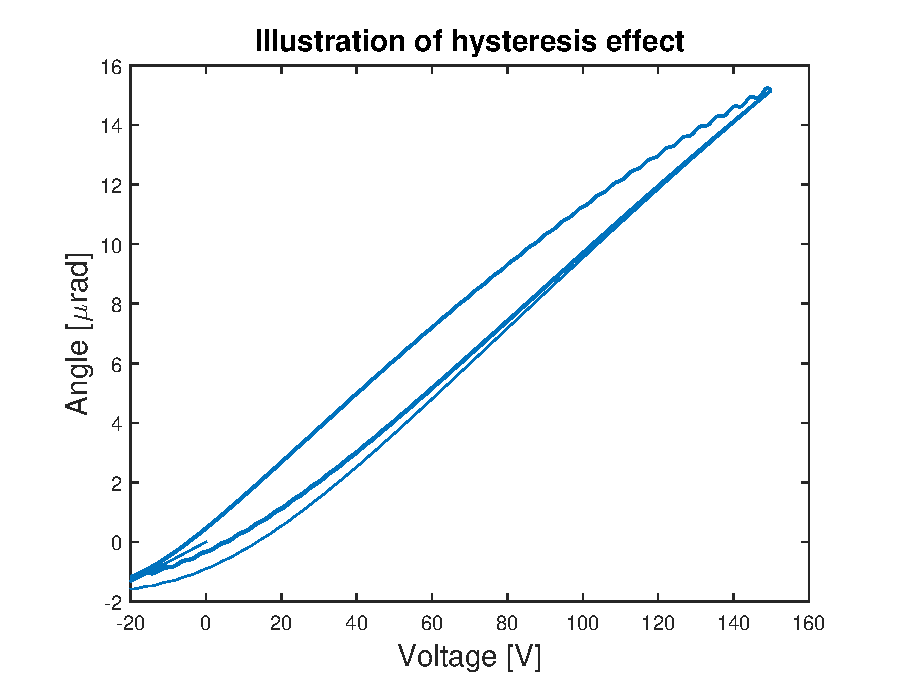
\includegraphics[width=0.5\textwidth]{fig/matlab/hysteresis.eps}
  \caption{\label{fig:hysteresis}Illustration of the hysteresis effect.}
\end{figure}

\subsection{Creep Effect}
The creep effect is another nonlinear effect that is present during the operation of piezoelectric actuators. The effect is a slow elongation or contraction of the actuator displacement over time, with a constant driving signal and is caused by thermal effects in the piezoceramics. Figure~\ref{fig:creep} illustrates the creep effect. One can see how the rotational stage slightly drifts in rotation after the applied negative step.

\begin{figure}[h]
  \centering
  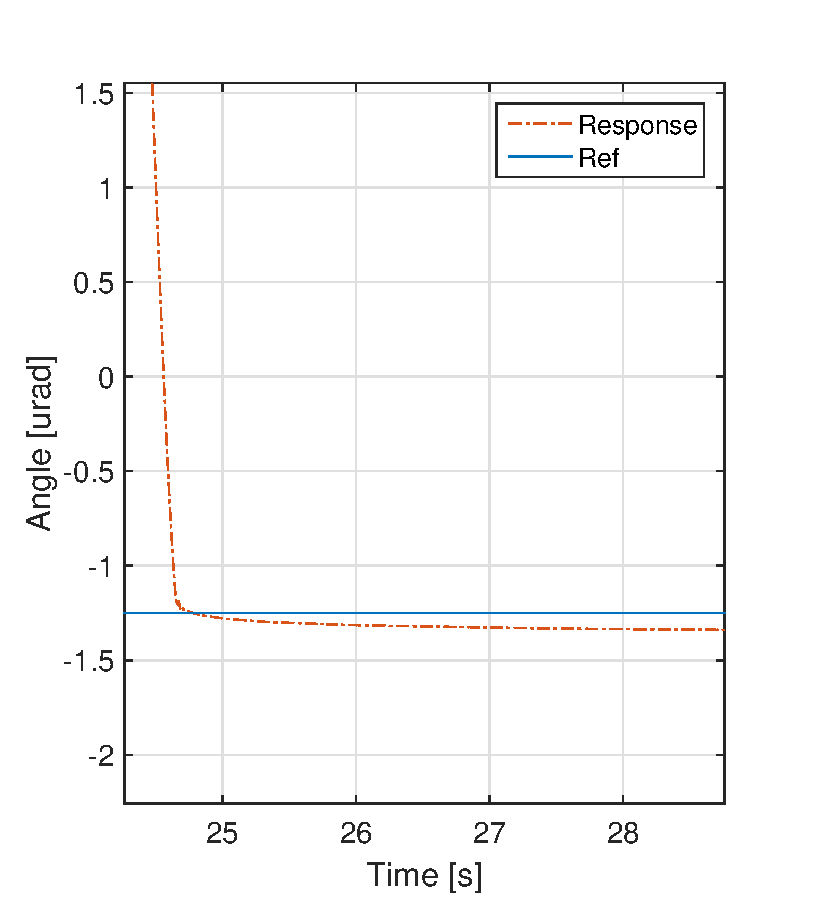
\includegraphics[width=0.5\textwidth]{fig/matlab/creep.eps}
  \caption{\label{fig:creep}Illustration of the creep effect. Note that the creep effect can last up to 10-15 minutes even if the plot only shows the development over 4 seconds.}
\end{figure}

The creep effect is in this project (and many others) effeciently suppressed by the feedback controller requiring no precise modeling and cancellation techniques.

\section{Rotational Stage Modeling}
The piezoactuated rotational stage is modelled by a Hammerstein structure, adopted by the authors in \cite{ButcherController:2015}, allowing them in principal, to decouple the nonlinear hysteresis from the linear system dynamics. The employed Hammerstein structure is depicted in Figure~\ref{fig:hammerstein} and consists of a \emph{Static Hysteresis} (rate independent) model and a \emph{Linear Dynamics} model. {\abbrPEA}s are known to show hysteretic behavior with a nonlocal memory (the current output does not only depend on the current input voltage but also on its history) as described in \cite{ButcherIdentification:2015}. This behvaiour is modeled by a generalised Maxwell-slip compensation model, described in \ref{sec:maxwell}. The extracted linear dynamics is identified using the described procedure in \ref{sec:linsys}

\begin{figure}[h]
  \centering %crop: left bottom right top
  \includegraphics[width=0.7\textwidth, trim=8cm 8cm 7.73cm 8cm, clip=true]{fig/matlab/hammerstein}
  \caption{\label{fig:hammerstein}Block diagram of the Hammerstein structure, consisting of two blocks in series, modeling the static hysteresis and the linear dynanamics, respectively.}
\end{figure}

\subsection{Maxwell-slip Model}
\label{sec:maxwell}
A generalized Maxwell-slip is used to model the hysteresis effect. It uses a parallell $n^{th}$ order elasto-slide element system with a friction force acting on each element, to create a nonlinear model. An elasto-slide element consist of a massless spring connected in series with a massless block that is subject to Coulomb friction. The model is summerized in the following equations and described more thourghly in \citep{Ru:2016}.

\begin{equation}
  \label{eq:maxwell_slip}
  F_i =
  \begin{cases}
    k_i(x - x_{bi}) & \quad \text{if }  k_i|x - x_{bi}| < f_i\\
    f_isgn(\dot{x}) \text{ and } x_{bi} = x - \frac{f_i}{k_i}sgn(\dot{x})  & \quad \text{else}\\
  \end{cases}
\end{equation}

\begin{equation}
  \label{eq:maxwell_sum}
  F = \displaystyle\sum_{i=1}^{n} F_i
\end{equation}

Where $F_i$ is (in terms of the rotational stage) the applied voltage, $x$ the rotaional displacement, $x_b$ blocked displacement and $k_i, f_i$ are unkown parameters where $i=1 \hdots n$ . The model parameters have been estimated by fitting the model to the major hysteresis loop, obtained by acquiring data from the system with a 0.5 Hz input driving signal as described in \cite{ButcherIdentification:2015,ButcherController:2015}. The result is presented in Figure~\ref{fig:maxwell} and Table~\ref{tab:maxwell} where $n=10$.

\begin{figure}[h]
  \centering
  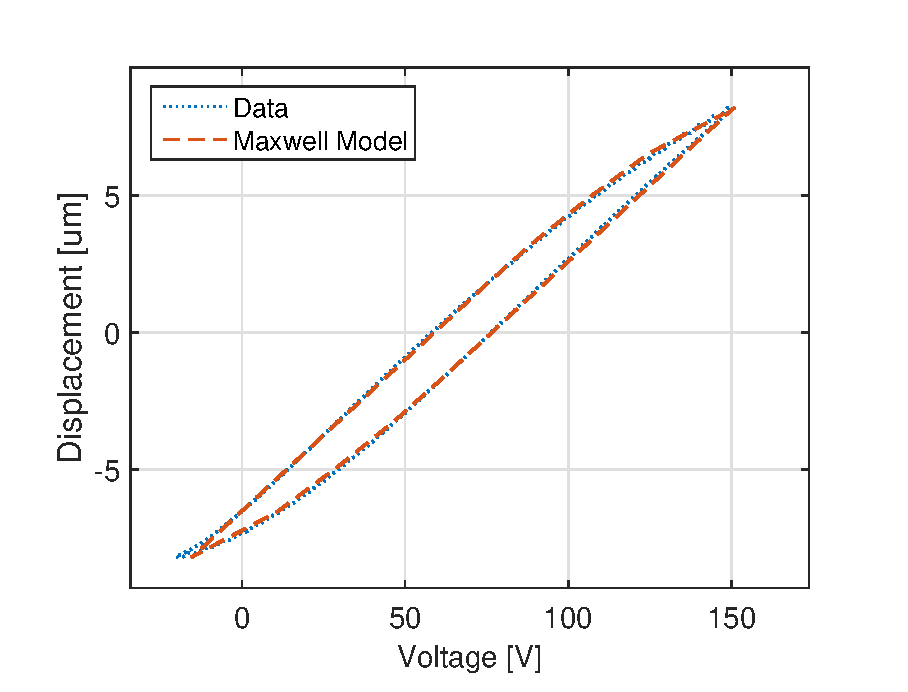
\includegraphics[width=0.5\textwidth]{fig/matlab/maxwell.eps}
  \caption{\label{fig:maxwell} The plot shows the model fit of the Maxwell slip model to the aquiered hysteresis of the rotational stage. The fit has a mean squared error of 1.1464.}
\end{figure}

\begin{table}[h!]
  \centering
  \begin{tabular}{| l | l | l |}
    \hline
    $i$ & $k_i$ & $f_i$ \\ \hline
    1 & 4.53 & 3.69 \\
    2 & 0.90 & 1.46 \\
    3 & 1.01 & 2.47 \\
    4 & 0.36 & 1.16 \\
    5 & $1.49 \times 10^{-6}$ & $4.28 \times 10^{-6}$ \\
    6 & $2.89 \times 10^{-7}$ & $1.41 \times 10^{-6}$ \\
    7 & $1.59 \times 10^{-7}$ & $9.10 \times 10^{-7}$ \\
    8 & $1.39 \times 10^{-7}$ & $9.10 \times 10^{-7}$ \\
    9 & $2.28 \times 10^{-7}$ & $1.67 \times 10^{-6}$ \\
    10 & $4.58$ & 37.30 \\
    \hline
  \end{tabular}
  \caption{\label{tab:maxwell} Identified parameters of the Maxwell slip model.}
\end{table}

\subsection{Linear System Identification}
\label{sec:linsys}
The extracted linear dynamics has been identified as an $6^{th}$ order Output-Error system using a \abbrPRBS as excitation signal, allowing for a valid extraction from the nonlinear dynamics. The system transfer function has been derived in discrete-time using the the System Identification Toolbox in Matlab. A more detail description of the procedure is available in \citep{ButcherController:2015}. Figure~\ref{fig:model} shows a comparision between the model and the real system in the frequency domain, where the Fast Fourier Transform (\abbrFFT) identification is calculated by dividing the \abbrFFT of the output with the \abbrFFT of the input.

 The transfer function of the model, discretized with a sampling time of \unit{0.5}{\milli\second}, is presented in \eqref{eq:tf}.

\begin{equation}
  \label{eq:tf}
  G_o(z) = \frac{21.05z^{-1} - 6.85z^{-2} + 8.52z^{-3} - 0.71z^{-4} + 9.30z^{-5}}{1 - 1.85z^{-1} + 1.09z^{-2} + 0.016z^{-3} - 1.32z^{-4} + 1.55z^{-5} - 0.48z^{-6}}
\end{equation}

\begin{figure}[h]
  \centering
  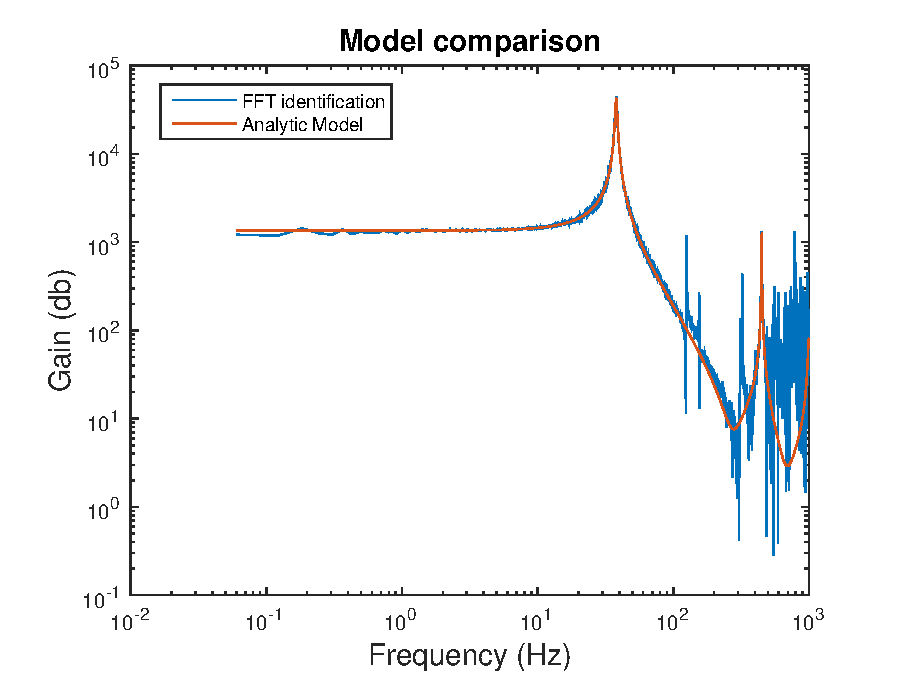
\includegraphics[width=0.5\textwidth]{fig/matlab/model.eps}
  \caption{\label{fig:model} The plot shows the model fit of the Maxwell slip model to the aquiered hysteresis of the rotational stage. The fit has a mean squared error of 1.1464.}
\end{figure}


\section{Present Control Approach}
The original controller for the rotational stage is a 2-\abbrDOF structure (feedback and prefilter). A schematic overview of the control loop is depicted in Figure~\ref{fig:present}, consisting of a controller block C, a prefilter F, a disturbance d and the linearized rotationalstage $G =G_oH^{-1}$, where $G_o$, $H^{-1}$ is the linear dynamics and the hysteresis compensator, respectively.

\begin{figure}[h]
  \centering %crop: left bottom right top
  \includegraphics[width=1\textwidth, trim=4cm 3cm 2.1cm 10cm, clip=true]{fig/matlab/present_controller}
  \caption{\label{fig:present}Block diagram of the present control loop, inlcuding controller, prefilter and hysteresis compensator.}
\end{figure}

The controller block (C) is a series combination of a \abbrPID controller, notch filter and a lead network, aiming to stabilize the system (\abbrPID), increase the sufficient phase margin (lead) and make the system robust to high frequency oscillations (notch). Since the bandwidth of the system is relatively low, $f_b = 58 Hz$ according to  Figure~\ref{fig:model}, it has been decided to exclude cancellation of the first resonance peak in order to keep the bandwith as high as possible and have a sufficient attenuation on the sensitivity function \citep{ButcherController:2015}. The PID controller, lead network and notch filter are all presented below in \eqref{eq:controller}.

\begin{subequations}
  \label{eq:controller}
\begin{alignat}{2}
  \label{eq:pre}
  & F = \frac{0.0029z - 0.0029}{z^3 - 2.91z^2 + 2.816 z - 0.91} \\
  \label{eq:pid}
  & C_{PID} = \frac{0.47z^2 - 0.94z + 0.47}{z^2 - 1.78 z + 0.78} \\
  \label{eq:lead}
  & C_{lead} = \frac{4.20 z^2 - 7.72z + 3.55}{z^2 - 1.67z + 0.69} \\
  \label{eq:notch}
  & C_{notch} = \frac{0.28z^4 - 0.62z^3 + 0.75z^2 - 0.59z + 0.26}{z^4 - 1.95z^3 + 1.39z^2 - 0.40z + 0.039}
\end{alignat}
\end{subequations}

% !TEX root = main.tex
\chapter{Control approaches}\label{cha:modelling}
This chapter presents the motivation and the theory behind each of the control approaches investigated in this thesis, including the present control loop.

\section{Present control loop}
The original controller for the rotaional stage is a PID controller which is used in combination with a pre-filter and a hysteresis compensator.

\section{Model Reference Adaptive Control}
An adaptive controller has the ability to adjust the system repsonse by updating the parameters of a feedback controller in real time, resulting in a controller that is less sensitive to changes in the model and aging of the system. One approach is to use a reference model to create the desired system response which the adaptive laws will aim for, this approach is known as the Model Reference Adaptive Controller (MRAC). This model does not require any prior knowledge about the model uncertainties, implying in a more straight forward way to implement precision control to nanopositioning systems. Moreover, this scheme allows for the use of a lower order model (in relation to the system model) since the online parameter estimation can be used sufficiently with a lower order model. The MRAC scheme can be extended to include perturbation estimation (MRACPE), giving the controller the ability to compensate for various unmodelled effects, including both linear and nonlinear perturbations. Nonlinear effect such as the hysteresis are treated as lumped perturbations to the nominal system model and can be compensated for in the same manner as linear, using the knowledge of the system and the previous measurement and outputsignal. The MRACPE also allows the maximum tracking error to be predefined.


\subsection{Perturbation Estimation}
Using a second order model, the adaptive laws can be derived as follows. Consider the system model stated in~\eqref{eq:sysmodel}.
\begin{equation}
  \label{eq:sysmodel}
  \ddot{x}(t) + \alpha_1\dot{x}(t) +  \alpha_0x(t) = \beta_0u(t) + f(t)
\end{equation}

where $x(t)$ denotes the output rotation at time t, $u(t)$ the input voltage at time t and $\alpha_1, \alpha_0, \beta_0 \in \mathbb{R}$ are known system constants. $f(t)$ is a function describing the unknown perturbations of the system, including the hysteresis and creep effect.

In order to estimate the perturbation function consider the following nonlinear system in one dimension, described more thoroughly in \cite{Elmali:1996}.

\begin{equation}
  \label{eq:perturbation}
  x^{(n)} = f(\mathbf{X}) + \Delta f(\mathbf{X}) + [B(\mathbf{X}) + \Delta B(\mathbf{X})]u(t) + d(t)
\end{equation}

where the $x^{(n)} \in \mathbb{R}$ denotes the $n$th order of time derivative, and $\mathbf{X} = $\\ $[x, \dot{x}, \hdots, x^{n-1}]^T\in \mathbb{R}^n$ denotes the state vector. $f(\mathbf{X})$ and $\Delta f(\mathbf{X})$ corresponds to a nonlinear term and its perturbation, $B(\mathbf{X})$ and $\Delta B(\mathbf{X})$
represents the control gain and its uncertainty, while $u(t)$ and $d(t)$ corresponds to the driving signal and the system disturbance, respectively.

By using Eq.~\eqref{eq:perturbation} one can express the perturbation $\Psi(t)$ as ~\eqref{eq:perturbation_2} and forming its estimate according to ~\eqref{eq:estimate} as follows.

\begin{equation}
  \label{eq:perturbation_2}
  \Psi(t) = \Delta f + \Delta Bu(t) + d(t) = x^{(n)} -f - Bu(t)
\end{equation}

\begin{equation}
  \label{eq:estimate}
  \Psi_{est}(t) = x_{cal}^{(n)} -f - Bu(t-Ts)
\end{equation}

where $x_{cal}^{(n)}$ denotes the calculated state vector, $T_s$ is the sampling time interval and $u(t-T_s)$ is the control input in the previus timestep. $u(t-T_s)$ is often approximated to $u(t)$ in practice which is valid approximation if $T_s$ is sufficiently small.

The state vector is, for simplicity and its computational efficiency, computed by a simple backward different equation depicted below.

\begin{equation}
  \label{eq:backward}
  x_{cal}^{(n)}(t) = \frac{x_{cal}^{(n-1)}(t) - x_{cal}^{(n-1)}(t-T_s)}{T_s}
\end{equation}

Applying ~\eqref{eq:estimate} to the model in~\eqref{eq:sysmodel} and setting $f = 0$ since the nonlinearities are treated solely as a distrubance gives the following perturbation estimation. Denote that $x(t)$ here is the sensor input, i.e. the measured yaw angle.

\begin{equation}
  \label{eq:perturbation}
  \hat{f}(t) = \ddot{x}_{cal}(t) + \alpha_1\dot{x}_{cal}(t) +  \alpha_0x(t) - \beta_0u(t-T_s)
\end{equation}

\subsection{Adaptive laws}
The objective of the adaptive laws is to calculate the control parameter so that they converges to ideal values resulting in a system response that matches the reference. The adaptive laws can be derived using Lyaponov theory which is outlined in this section. Consider the second order reference model below

\begin{equation}
  \label{eq:refmodel}
  \ddot{x}_m(t) + a_1\dot{x}_m(t) +  a_0x_m(t) = b_0u_d(t)
\end{equation}

where $x_m(t)$ denotes the output rotation, $u(t)$ the input voltage and $a_0, a_1, b_0$ are known positive constants.

The tracking error is defined as $e=x-x_m$. Recalling~\eqref{eq:sysmodel}, replacing $f(t)$ with the estimation $\hat{f}(t)$ and subtracting it from the ~\eqref{eq:refmodel} gives the following expression, more details can be found in~\ref{Qingson:2016}.

\begin{equation}
  \label{eq:refmodel}
  \ddot{e}(t) + a_1\dot{e}(t) + a_0\dot{e}(t) =  (a_1-\alpha_1)\dot{x}(t) + (a_0-\alpha_0)x(t) - b_0u_d(t) - \beta_0u(t) + \hat{f}(t)
\end{equation}

This can easily be written on state-space form as follows.

\begin{equation}
  \label{eq:refmodel}
  \ddot{e}(t) + a_1\dot{e}(t) + a_0\dot{e}(t) =  (a_1-\alpha_1)\dot{x}(t) + (a_0-\alpha_0)x(t) - b_0u_d(t) - \beta_0u(t) + \hat{f}(t)
\end{equation}

\begin{theorem}
  Hello
\end{theorem}






\begin{chapter-appendix}
  \label{ap:lyaponov}

\section{MRACPE}


\end{chapter-appendix}

% !TEX root = main.tex
%preliminära resultat som kan demonstreras vid halvtidskontroll
\chapter{Results}\label{cha:result}
This section describes the results considering performance, robustness and stability with respect to the different control approaches. All approaches will first be benchmarked with the present control approach and presented individually in the following subsections. A comparison between all approaches is presented in the end of this chapter.

\section{Benchmark test}
Each of the control approaches have been evaluated with respect to robustness to model errors, disturbance rejection, closed loop bandwidth and response to step, ramp and sinusoidal input, all summarized below. The prospective challanges, described in \ref{sec:prospectiveChallanges} shall be kept in mind while reading the results. Since the required ramprates are relatively low, the disturbance rejection and the robustness to model errors are more of interest when evaluating each method.

\begin{itemize}
\item {\bf Step, ramp and periodical tracking} - A step, ramp and periodic input is applied on the input to benchmark the tracking capability of the controller.
\item {\bf Disturbance rejection} - Modified step responses with added noise is applied to the input to benchmark how sensitive the system is to system disturbances.
\item {\bf Robustness to model errors} - During operation with a periodic input signal, the dynamical model is changed and the output is studied to characterize the robustness to model errors. This test is of importance since this is exactly what happens when the linear stage moves the rotational stage further out.
\end{itemize}

\section{Simulation Results}
For the comparison with the present control approach, all evaluated controllers were discretized with a sampling frequency of 2kHz. The high order system model in \eqref{eq:tf} was used to model the rotational stage dynamics linear dynamics. The nonlinear dynamics, creep and hysteresis, were neglected in the simulations, assuming perfect inverse hysteresis cancellation and a sufficient closed loop to compensate for the creep effect.

\subsection{Model Reference Adaptive Control}
Even though the rotaional stage has been modelled by \eqref{eq:tf}, a second order model approximating the higher order system was used in the adaptive control laws to keep the computational burden low. The discretized reference model can be seen in \eqref{eq:sys_gm} and all parameters and tuning variables is summerized in Table~\ref{tab:adaptive_param}. The controller is tuned to be robust to input disturbances and model changes. The set of parameter presented in Table~\ref{tab:adaptive_param} is not an optimal set but a decent set of parameters that maintains stability for stepsizes below 20mrad.

\begin{equation}
  \label{eq:sys_gm}
  G_m(z) = \frac{7.9z + 6.7}{1313z^{2} - 2095z + 796.4}
\end{equation}

\begin{table}[h!]
  \centering
  \begin{tabular}{| l | l |}
    \hline
    Parameter & Value \\ \hline
    $T_s$ & $5 \times 10^{-4}$ \\
    $\alpha_0$ & $5.7 \times 10^{4}$ \\
    $\alpha_1$ & $7.2$ \\
    $\beta_0$ & $7.5 \times 10^{7}$ \\
    $a_0$ & $5.7 \times 10^{4}$ \\
    $a_1$ & $1 \times 10^{3}$ \\
    $b_0$ & $7.5 \times 10^{7}$ \\
    $\eta_0$ & $3 \times 10^{-2}$ \\
    $\eta_1$ & $1 \times 10^{-1}$ \\
    $\eta_2$ & $1 \times 10^{-10}$ \\
    $\eta_3$ & $1 \times 10^{-17}$ \\
    $\epsilon$ & $1 \times 10^{-8}$ \\
    $Q$ & $diag(1 \times 10^{10}, 1 \times 10^{-3})$\\
    \hline
  \end{tabular}
  \caption{\label{tab:adaptive_param} Parameters of the system model and the tuned adaptive controller.}
\end{table}

Figure~\ref{fig:step_adaptive} shows the step repsonse to different stepsizes. Here it is clear that the system becomes unstable if the stepsize $\geq$ \unit{26}{\milli\radian}. The controller has been tuned to handle the maximum stepsize, i.e the rotational range of \unit{20}{\milli\radian}, which results in a longer rise time for the smaller stepsizes. Note that the responses are produced with initial values $k_i = 0$, if the initial values would be set to the values that $k_i$ settles to, a faster step response could be expected. This can be seen in Figure~\ref{fig:periodic_resp} where the controller performs better for the second period.

\begin{figure}[h!]
  \centering
  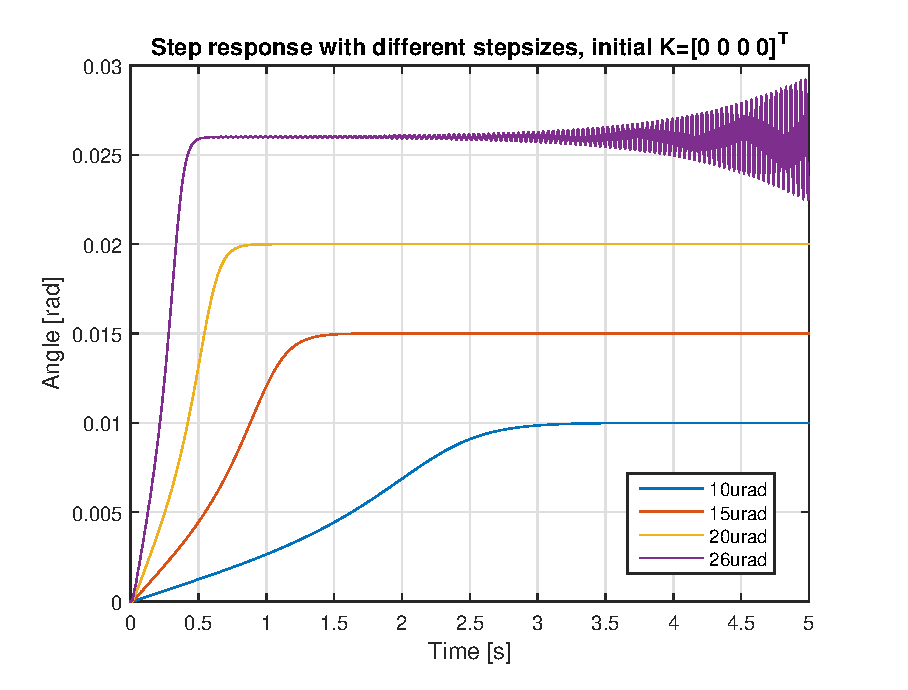
\includegraphics[width=0.7\textwidth]{fig/matlab/stepresponse.eps}
  \caption{\label{fig:step_adaptive} Step responses to stepsizes of 10, 15, 20 and 26 mrad.}
\end{figure}

The adaptation process of the control parameters $k_i$, for a stepresponse resulting from a 20mrad step, can be seen in Figure~\ref{fig:adapt_process}. All of the coefficients have converged within 1 second.

\begin{figure}[h!]
  \centering
  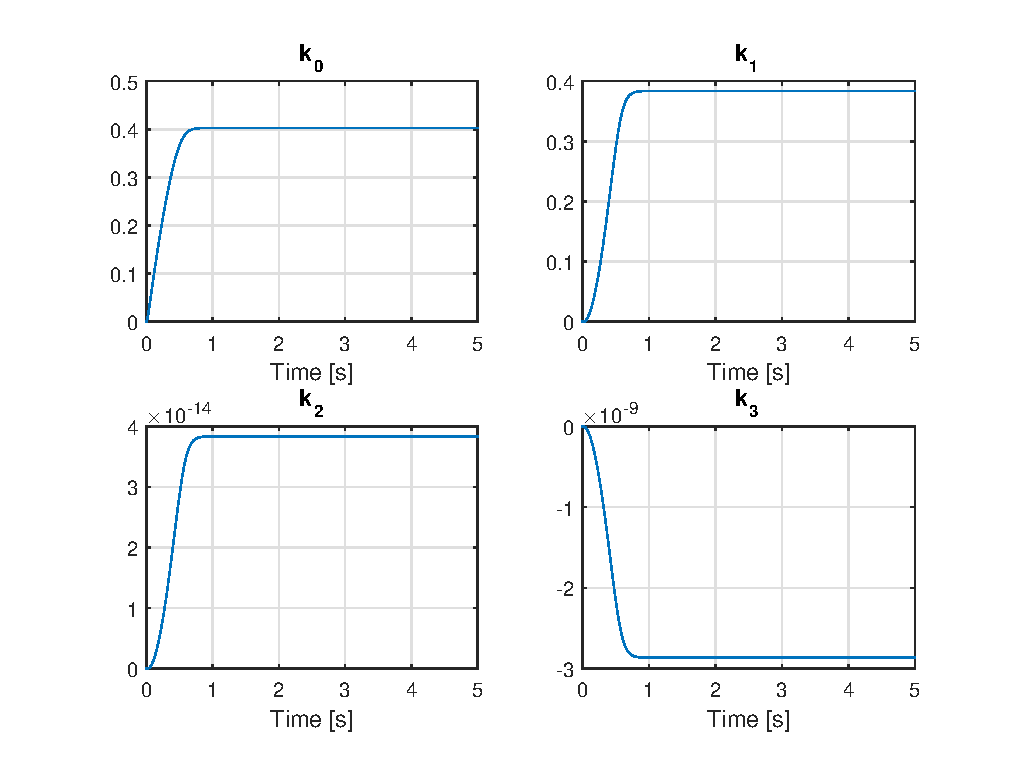
\includegraphics[width=0.7\textwidth]{fig/matlab/k.eps}
  \caption{\label{fig:adapt_process} Adaptation process of control parameters $k_i$ with a 20 mrad step.}
\end{figure}

To illustrate the adaptation process better, a periodic response is depicted in Figure~\ref{fig:periodic_resp}, here it is clear that after the adaptation process is finished the controller performs better for the second and third period. One can see that the adaptation process is slower for the periodic response corresponding to the amplitude of \unit{10}{\milli\radian}, hence the lower the step, the longer the adaptation time. The present controller performs well for all amplitudes.

\begin{figure}[h!]
  \centering
  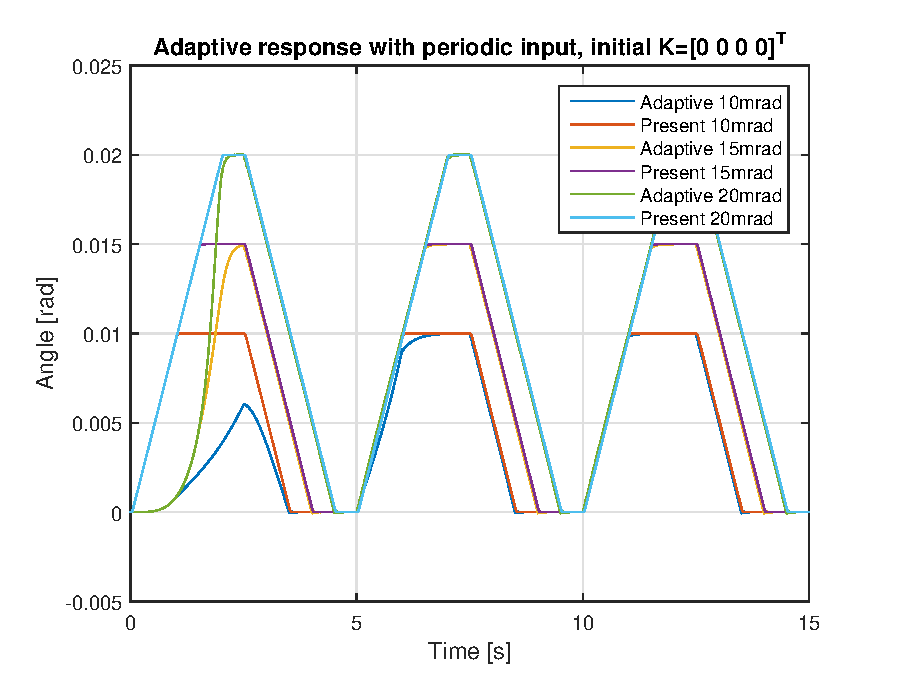
\includegraphics[width=0.7\textwidth]{fig/matlab/periodicresponse.eps}
  \caption{\label{fig:periodic_resp} Periodic responses for the adaptive and present controller with amplitudes of 10, 15, 20 mrad.}
\end{figure}

The tracking error corresponding to the \emph{Adaptive 20mrad} and \emph{Present 20mrad} in Figure~\ref{fig:periodic_resp} can be seen in Figure~\ref{fig:adapt_trackingerror}. The adaptive controller performs better than the present controller after the adaptation process has finished.
\begin{figure}[h!]
  \centering
  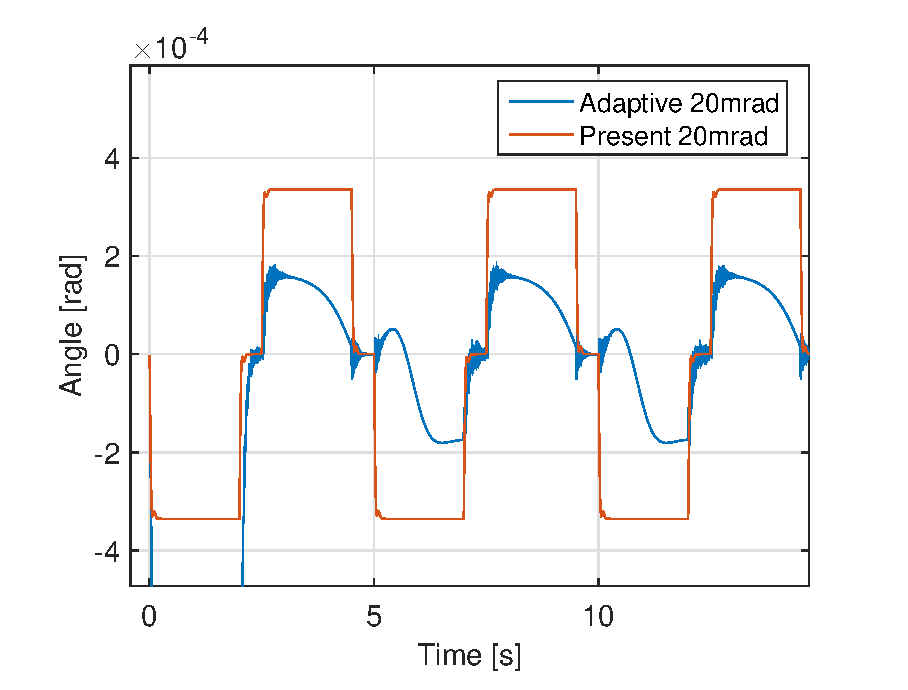
\includegraphics[width=0.7\textwidth]{fig/matlab/trackingerror.eps}
  \caption{\label{fig:adapt_trackingerror} Tracking error (difference between reference and output) for the periodic response from an input signal with an amplitude of 20 mrad.}
\end{figure}

A periodic repsonse with model parameter drift is presented in Figure~\ref{fig:modeldrift}. It shows how the adaptive controller manages to adapt to the change in the system dynamics, while the present controller fails to do so, resulting in an unstable system. The change of the model was performed over 2 seconds, resulting in a movement of the first resonance peak, from 38 Hz to 66 Hz in frequency and from 30.1 dB to 23.5 dB in magnitude. Note that the change of the model is relatively big and for a smaller movement of the resonance peak, the present controller could still be sufficient as illustrated in Figure~\ref{fig:modelerror}.
\begin{figure}[h!]
  \centering %crop: left bottom right top
  \subfloat[][\label{fig:modeldriftresponse}Periodic response with model parameter drift.]{
  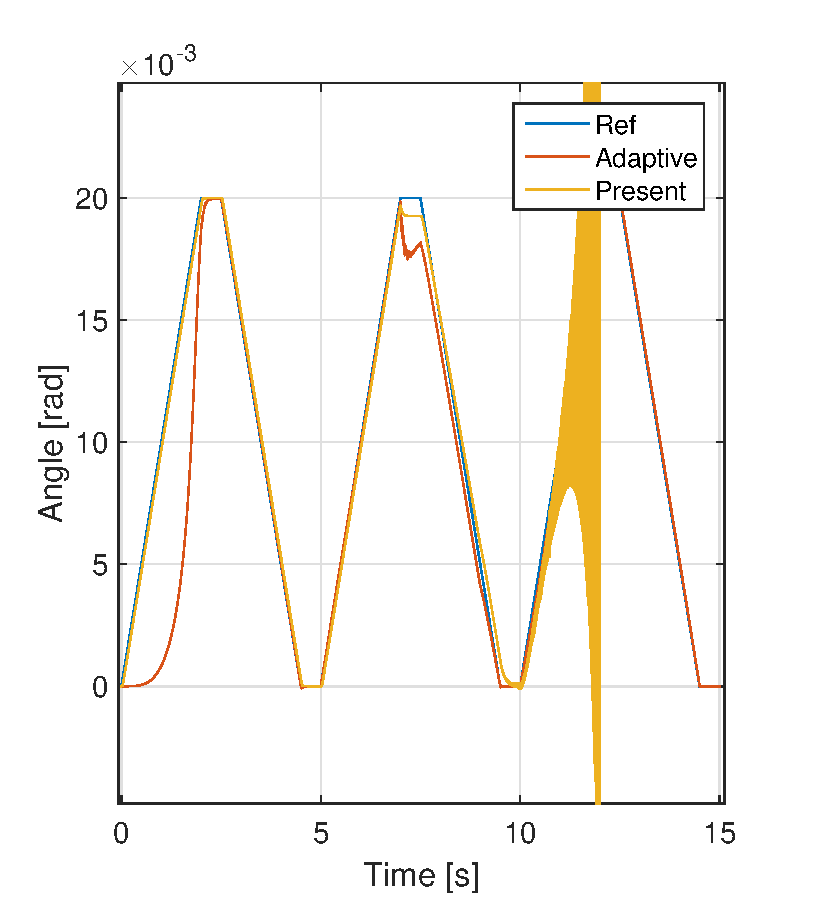
\includegraphics[width=0.45\textwidth]{fig/matlab/driftofmodelparameterover2s.eps}}
  \qquad
  \subfloat[][\label{fig:modeldriftbode}Original model (G) and the resulting model after drift ($G_mod$).]{
  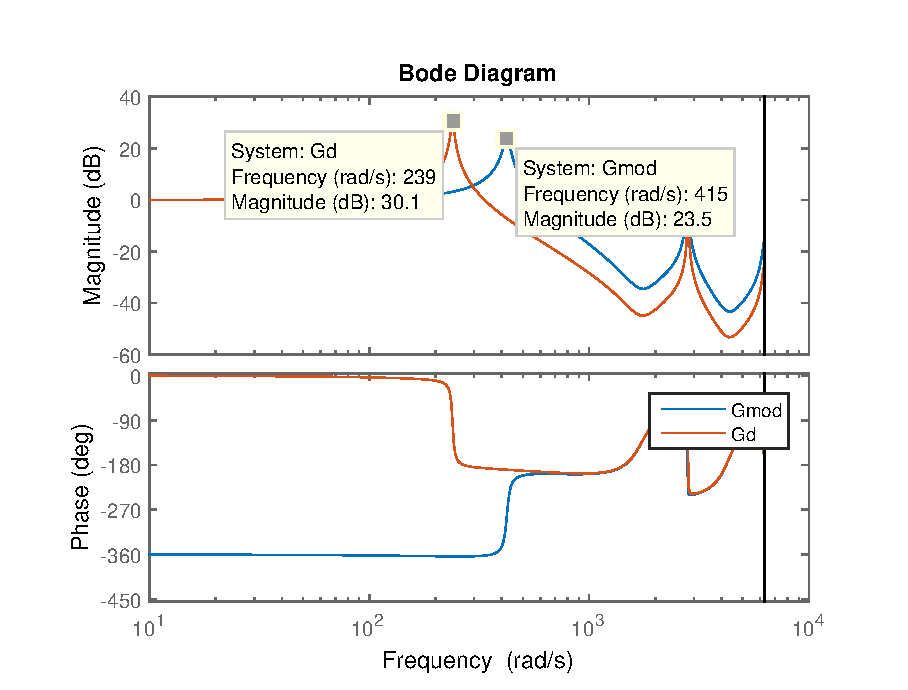
\includegraphics[width=0.45\textwidth]{fig/matlab/bode_drift_pole.eps}}
  \caption{\label{fig:modeldrift} Shows the robustness to model changes over time. The model error is increased linearly from $t=7s$ to $t=9s$. The resulting responses is shown in (a) while the model change is presented in (b).}
\end{figure}

\begin{figure}[h!]
  \centering %crop: left bottom right top
  \subfloat[][\label{fig:modelerrorresponse}Periodic response with model parameter drift.]{
  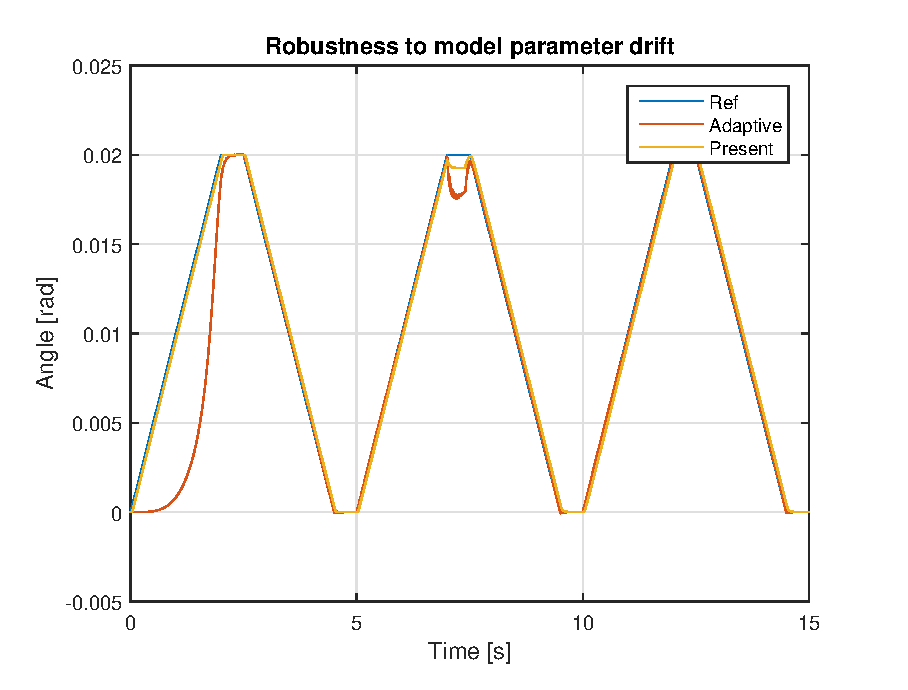
\includegraphics[width=0.45\textwidth]{fig/matlab/modelerrorperiodic.eps}}
  \qquad
  \subfloat[][\label{fig:modelerrorbode}Original model (G) and the resulting model after drift ($G_mod$).]{
  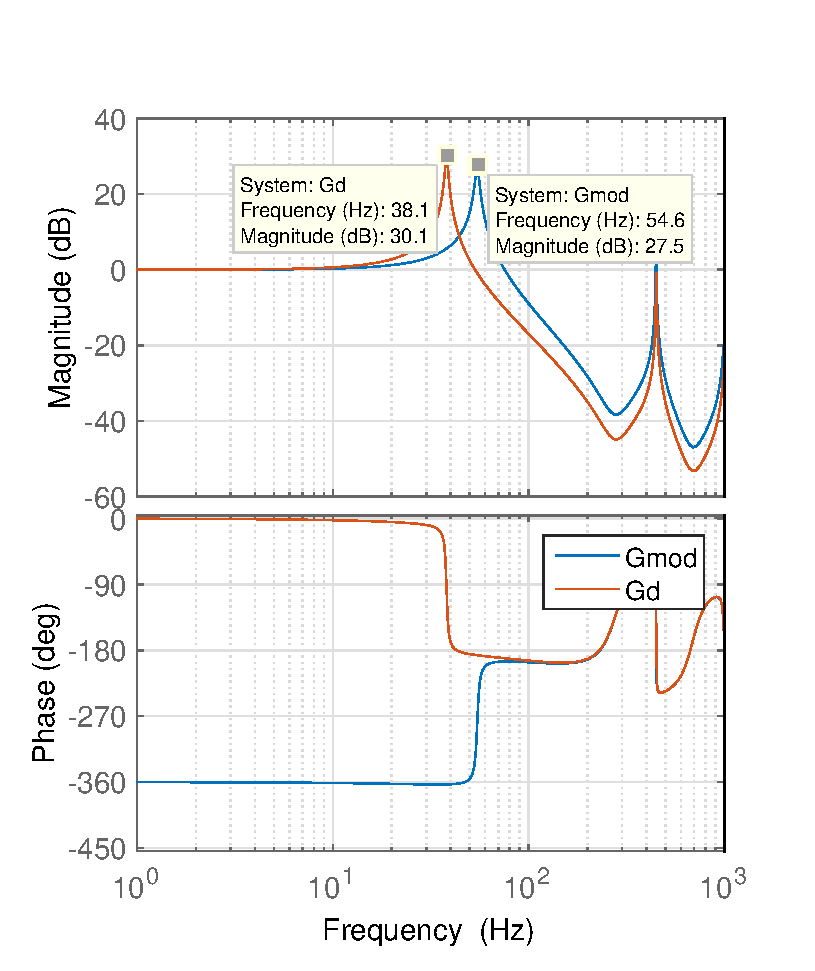
\includegraphics[width=0.47\textwidth]{fig/matlab/bode_modelerror_pole.eps}}
  \caption{\label{fig:modelerror}Shows the robustness to model changes over time. The model error is increased linearly from $t=7s$ to $t=9s$. The resulting responses is shown in (a) while the model change is presented in (b).}
\end{figure}

In the case in Figure~\ref{fig:modelerror} the resonance peak is only moved to 45.5 Hz and the present controller is sufficient to suppresses the disturbance. It even does it more efficiently than the adaptive controller.

Figure~\ref{fig:distrejection} shows the disturbance rejection capability of the controllers. A small glitch was added on the input to see if the controllers would attenuate it sufficiently. The adaptive controller performed worse than the present controller both with and without prefilter. The present controller managed to attenuated the highest peak of the glitch by 3 times more than the adaptive with prefilter and 5 times more than the adaptive without prefilter.  The settling time was also approximately 12 times worse for the adaptive controllers.

\begin{figure}[h!]
  \centering %crop: left bottom right top
  \subfloat[][\label{fig:dist}Step response]{
  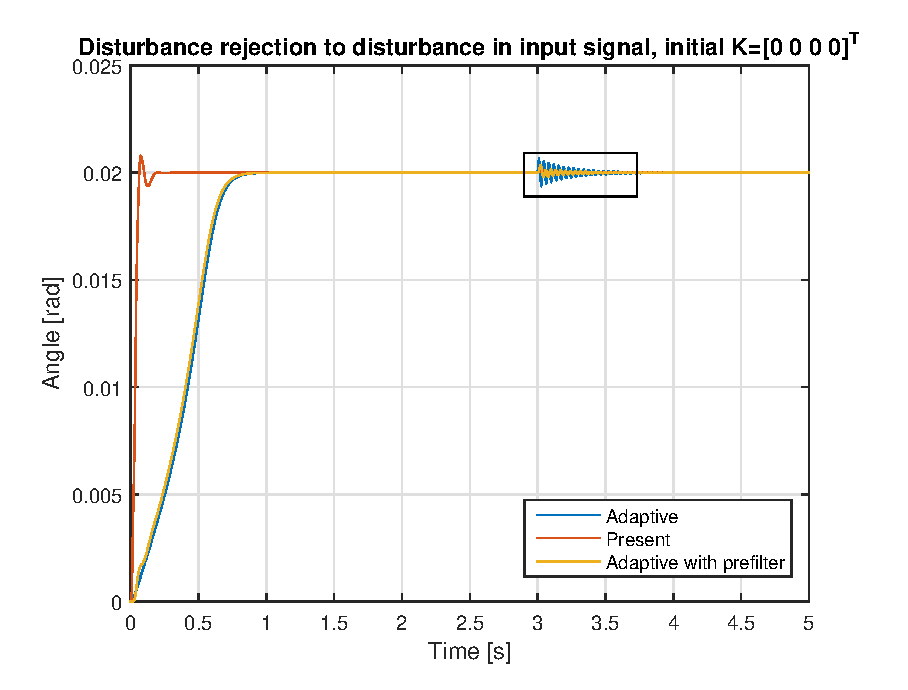
\includegraphics[width=0.45\textwidth]{fig/matlab/distrejection.eps}}
  \qquad
  \subfloat[][\label{fig:distzoom}Zoom in on disturbance]{
  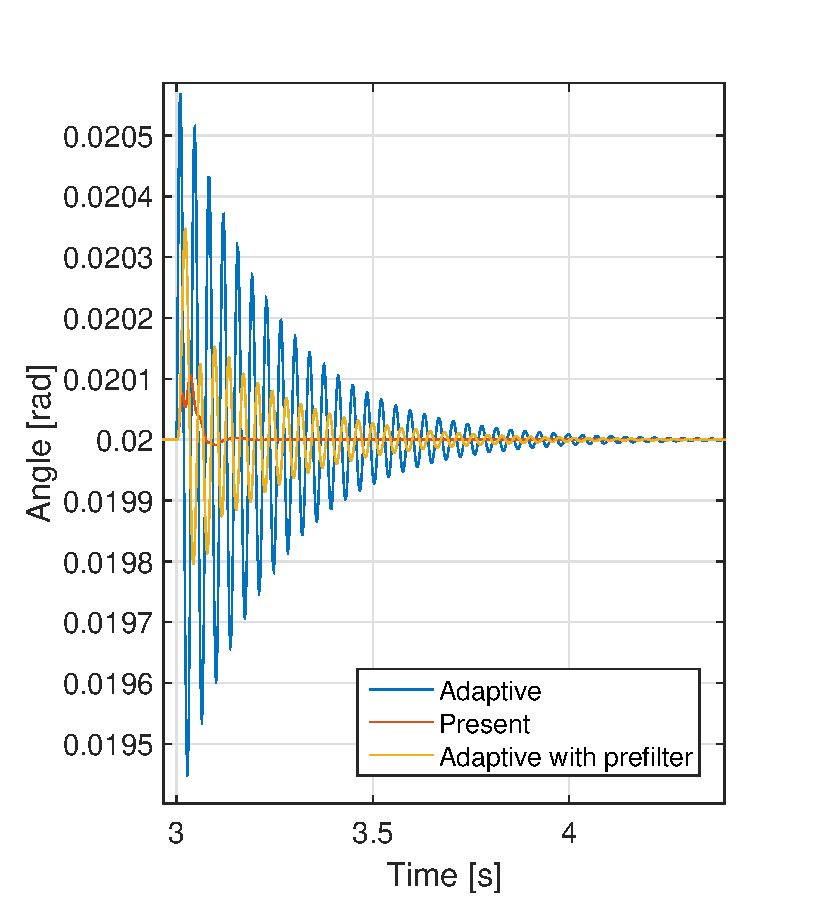
\includegraphics[width=0.45\textwidth]{fig/matlab/distrejection_zoom.eps}}
  \caption{\label{fig:distrejection} Shows how well the controller attenuates a disturbance glitch (amplitude of $5.1 \times 10^{-3}$) added to the input signal at $t=3s$. The whole step response is shown in (a) while a zoom in on the boxed area in (a) is presented in (b).}
\end{figure}

\section{Experimental Results}
\subsection{Setup}
The experiments have been conducted on the considered rotational stage described in Section~\ref{sec:rotational_stage}. A National Instruments PXI communicates with the Collimator and the rotaional stage, responsible for acquisition and control. To drive the rotaional stage it outputs a voltage between [-1, 7.5] V, this is amplified by a linear amplifier with a gain of \unit{20}{\volt/\volt} resulting in a [-20, 150] V signal input on the rotaional stage. The yaw angle, measured by the interferometric system is converted and sent to the PXI. The control loop is running at \unit{2}{\kilo\hertz}.

%Sätt av ett kort kapitel sist i rapporten till att avrunda och föreslå rikningar för framtida utveckling av arbetet.
% !TEX root = main.tex
\chapter{Conclusions and Future work}\label{cha:conclusion}

\section{Conclusions}

As seen in the zoom-in, the \abbrIRC is slightly more damped but has a high frequency ringing in 448Hz, the same frequency as the model's second resonance peak. In reality it would be plenty of  higher resonance (all are not modeled) that will lead to more ringing and bad disturbance rejection. 
\section{Future work}


% THESIS PLAN
% % !TEX root = main.tex
%en preliminär problemformulering satt i relation till litteraturbasen
\chapter{Introduction}\label{cha:intro}

\section{Background}
High precision positioning systems are vital in e.g. scanning tunneling microscopes (\abbrSTM), atomic force microscopes (\abbrAFM) and in semiconductor lithography. In \abbrAFM, for instance, high precision positioning is required to control the vertical position of the scanning probe to keep the force constant between the sample surface and the probe tip. An topographical image of the sample is obtained by raster-scanning the probe over the sample surface and plotting the vertical displacement against the probe's x-y position. A positioning system that keeps the force constant down to an atomic-scale resolution is thus inevitable in order to obtain a high resolution image without damaging the sample \citep{SurveyOfControlIssues:2007}.

The piezoelectric effect is a phenomenon that arises in certain solid materials when an electric potential is generated in response to applied mechanical stress. The effect was first discovered by Jacques and Pierre Curie in 1880 when they found that applying pressure to a quarz crystal generates electrical potential. Today, the effect is commonly encountered in daily life and utilized in for example lighters, buzzers and loudspeakers.

Smart materials such as piezoelectric and magnetostrictive materials are nowadays commonly used in precision actuators due to their ability to convert electrical energy into mechanical energy. Piezoelectric materials have been commercially available for almost 45 years and have become indispensable for the nanopositioning industry \citep{Piezo:2008}. In cases where a relatively small displacement range is required (travel ranges up to \unit{500}{\micro\meter}) a piezo electric device is the actuator of choice due to its fast response, high resolution and its ability to generate large mechanical forces for small amounts of power in compact designs \citep{SurveyOfControlIssues:2007}.

The Equipment Controls and Electronics section in the Engineering Department at \abbrCERN (European Organization for Nuclear Research) is developing a high precision positioning system for the control of a piezo-actuated rotational stage used in the UA9 Crystal Collimation study. The stage uses a piezo electric linear stack actuator to displace a flexible lever arm mechanism which generates the rotational movement.

\section{Purpose and Goal}
Crystalline solids have the ability to constrain the directions that particles take as they pass through, this is commonly called the "channelling" property. The UA9 collaboration at \abbrCERN is investigating how tiny bent crystals can help to steer particle beams in modern hadron colliders such as the Large Hadron Collider (\abbrLHC) \citep{WebsiteUA9:2016}. In high energy colliders, such as the \abbrLHC, particles tends to drift outwards creating a beam halo. These particles surrounding the beam, can be lost and cause damage to sensitive parts in the accelerator. By using bent crystals, halo particles can be efficiently extracted from the beam and collected by absorbers further away, reducing the complexity of the system. One major difficulty that arises is that the higher the energy of the particle, the lower the angular acceptance for channeling. Hence, a high precision positioning mechanism with a high angular accuracy is required. The rotational stage (with a range of \unit{20}{\milli\rad}) is of necessity to be able to track reference trajectories at ramp rates of \unit{100}{\micro\radianpersecond} and reject external disturbances (e.g. from the linear axis movement) to maintain a maximum tracking error of $\pm$\unit{1}{\micro\rad}.

This project aims to identify the possible control approaches that could be applicable to this problem to achieve the desired performance.

\section{Prospective challenges}
First of all, piezoelectric  actuators show strong nonlinear properties such as hysteresis and creep (drift), which have to be compensated for. Moreover, the mechanical flexural structure in combination with the piezo electric characteristics leads to a highly resonant structure, making it difficult to achieve the desired performance while operating the rotational stage within noisy environments with external disturbances such as ground vibrations. Furthermore this rotational stage is mounted on a linear stage which is composed of a leadscrew, a stepping motor and a gearbox. The linear movement adds additional perturbations to the rotational stage due to imperfections in the leadscrew and detent torque and stepping nature of the motor. Finally the system dynamics also show linear position and voltage level dependence requiring a controller that is robust to such variations.

One attempt to achieve the desired performance has already been made. The proposed controller, presented in \citep{ButcherController:2015} delivers reasonable performance but does not fulfill the requirements during linear axis movement. The authors proposes a PID controller in combination with a lead-, notch- and prefilter. The controller also uses a hysteresis compensator to mitigate the nonlinear behaviour. The controller has shown high disturbance rejection at the first resonance peak as well as good tracking performance.

\section{Outline}
This thesis plan presents an overview of the thesis, including method, literature base and expected results. A literature review is presented in  Chapter~\ref{cha:litreview}. The method and work flow of this thesis as well as a brief timeplan is given in Chapter~\ref{cha:method}. In Chapter~\ref{cha:result} the results that can be expected half way through the project are discussed while a brief summary of the thesis can be found in Chapter~\ref{cha:conclusion}.

% \include{plan/plan_litreview}
% % !TEX root = main.tex
% en preliminär beskrivning av angreppssätt
\chapter{Method}\label{cha:method}
This thesis will identify possible control approaches that could be applicable to the rotational stage at \abbrCERN in order to meet the performance requirements. The work is divded into three major subblocks; Identification of control approaches, Simulations and Implementation on real device.


\section{Identification of control approaches}
First of all, a brief analysis of the already developed controller will be done in order to point out the drawbacks and determine which controller qualities that have to be improved in order to achieved the desired performance during linear movement of the system. Moreover will a comprehensive literture study be done to understand the dynamics and identify possible control approaches. The main work will then consist of investigating different control approaches such as feedforward, H-infinity, iterative or state feedback control.

\section{Simulations}
After identifying a handful control approaches that could be applicable to this problem, simulations and implementaion will be done in Matlab and Simulink. The most promising approaches will be benchmarked in simulations and compared to the existing algorithm.

\section{Implementation on real device}
Finally, the most promising alternative will be implemented and tested on the real rotational stage. This will be done by implementating the control agorithm in Labview. The algorithm will run on a National Instruments PXI which will send the control signal and read the sensordata from the interferometer system.

\section{Timeplan}
%en tidplan för examensarbetets genomförande inklusive planerade datum för halvtidskontroll och framläggning
Figure~\ref{fig:timeplan} shows the timeplan for the master thesis project. \emph{HP} and \emph{FP} stands for halftime presentation and fulltime presentation, respectively. In addition to the master thesis work, some hardware testing will be carried out from time to time, throughout the whole thesis period.

\begin{figure}[h] %tbp
 \centering %crop: left bottom right top
 \includegraphics[trim=1cm 12cm 5cm 5.5cm, clip=true, scale=0.42]{fig/timeplan}
 \caption{\label{fig:timeplan}%
 Master Thesis timeplan, HP = Halftime presentation, FP = Fulltime presentation}
 \end{figure}

% % !TEX root = main.tex
%preliminära resultat som kan demonstreras vid halvtidskontroll
\chapter{Result}\label{cha:result}
This section describes future results that could be expected half way through the project.

\section{Control Approaches}
Half way through the project, all control approaches that have been identified should be presented here. Furthermore, all control approaches that at the time have been simulated will be presented with a schematic structure, transfer functions or state space model, a design analysis of the closed loop system and additional plots for illustration of the trajectory tracking capability and the robustness.

\section{Benchmark tests}
Benchmark tests will be carried out on all simulated control approaches and presented here. Comparisons between the new control approaches and the existing algorithm with respect to disturbance rejection, trajectory tracking and closed loop bandwidth will be illustrated in this section with plots and tables.

% %Sätt av ett kort kapitel sist i rapporten till att avrunda och föreslå rikningar för framtida utveckling av arbetet.
% !TEX root = main.tex
\chapter{Conclusion}\label{cha:conclusion}

This thesis aims to identify, simulate and implement a suitable control approach for a piezo actuated rotational stage at \abbrCERN. The rotational stage is to be used within the UA9 project to position a bent crystal (which will steer particle beams) with a high accuracy. Several control approaches will be simulated in order to find a controller that meet the requirements. The best performing approach will be implemented and tested on the real device. 


% \part*{Appendix}
% \appendix
% %
% \chapter{definitions}\label{cha:definition}

\section{Test}

% \clearemptydoublepage

\backmatter

\bibliography{IEEEfull,myrefs}

\printindex

\end{document}
